\subsection{Design and Architecture}
The attacks of Section~\ref{sec:attacks} can be classified into two groups which have to be handled separately in order to increase security on the target platform. Attacks to the process virtual memory that have to use \gls{WPM}, which form the first group and attacks that are relying on a \gls{DLL} load during their initialization to execute their malicious code, which form the second group. This classification makes it possible to design effective countermeasures that can not be bypassed by attacks. The classification into the two groups, \gls{DLL} and \gls{WPM}, is used to for the architecture design. Figure~\ref{fig:interaction} shows the interacting components in an abstract representation. \emph{Windows} offers three entry points that will get called by the kernel, whenever a process is started, opened or a \gls{DLL} is loaded. The registered callback functions will then need to do several checks on the given information and based on this allow or deny execution.
\begin{figure}[h]
\centering
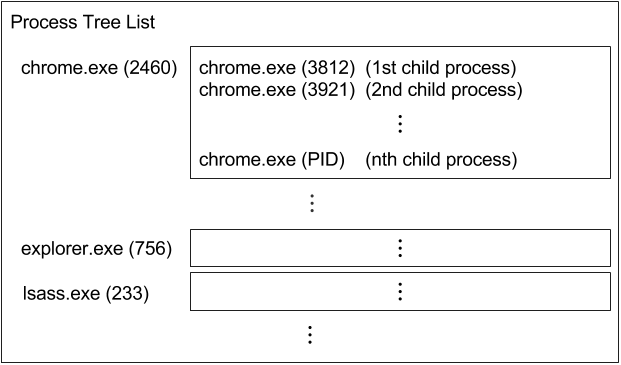
\includegraphics[scale=0.6]{sections/implementation/listoflists.png}
\caption{The process tree structure. A list of parent processes with their children}
\label{fig:listoflists}
\end{figure}
\begin{figure}[!p]
\centering

\includegraphics[angle=90,scale=0.6]{sections/implementation/interaction.png}
\caption{The interaction of the drivers components}
\label{fig:interaction}
\end{figure}
\paragraph{Process Tree Structure}
The \syscall{PsSetCreateProcessNotifyRoutine} callback function is called whenever a process is created or destroyed. Accordingly, whenever this callback function is executed, the process is inserted into the process tree structure on process creation, and removed from the process tree structure on process deletion. The process tree hereby maintains a list of lists, which is shown in Figure~\ref{fig:listoflists}.
Each list separates the processes parents with their children from other processes. If the process tree gets queried for a specific \gls{PID} the parent \gls{PID} gets returned. To illustrate this interaction, the data of Figure~\ref{fig:listoflists} is used for an example. If the process tree is queried with \gls{PID} 3812, a lookup in the process tree occurs to find a process with \gls{PID} 3812. In this case, the process is a child of chrome.exe with \gls{PID} 2460.
Because process 3812 is a child process, its parent 2460 is returned. For a second example, consider the process tree being queried for \gls{PID} 2460. Another lookup is done and a process with \gls{PID} 2460 is found. Because 2460 is a parent process, the process tree structure returns the value 2460.

\paragraph{WPM Component}
To prevent the group of \gls{WPM} attacks, a \gls{WPM} callback is registered which checks if the given \gls{PID} is in a whitelist. If it is not, the request is denied by removing the required permissions to execute \gls{WPM} attacks. Because \glspl{PID} are dynamically assigned by the kernel and the possibility of reusing \glspl{PID}, a internal structure, a process tree, needs to be maintained. This thus adds communication between the three callback functions and the process tree as seen in Figure~\ref{fig:interaction}.

\paragraph{DLL Component}
The last callback function of Figure~\ref{fig:interaction}, \syscall{PsSetLoadImageNotifyRoutine}, is called by the \emph{Windows} kernel whenever a \gls{DLL}- is loaded. The callback routine queries the process tree structure for a given \gls{PID} to see if this is a chrome.exe process. If it is a chrome.exe process, the callback generates a hash of the \gls{DLL} file, compares it to a whitelist and if a match can not be found takes action to prevent \gls{DLL} loading.